\documentclass[a4paper,10pt,xcolor=pdftex,dvipsnames,table]{beamer}
\mode<presentation>{%
		\usetheme{Antibes}%
		\usecolortheme{wolverine}
%		\usecolortheme{beaver}
%		\usecolortheme{crane}
%		\usecolortheme{whale}
%		\usefonttheme{structuresmallcapsserif}
%		\usefonttheme[onlysmall]{structurebold}				% use smallcaps in bold structures (not everywhere)
%		\usefonttheme[frametitle]{structuresmallcapsserif}
%		\usetheme[headline=sections,frametitle=normal,titlepage=picture]{progressbar}
%		\useinnertheme{progressbar}
%		\useoutertheme{progressbar}
        \useoutertheme{progressbar}
        \useinnertheme{rectangles}    % circles, inmargin, rectangles, rounded
%                \newcommand{\includeoptional}{false}
        \newcommand{\includeoptional}{true}
		\setbeamertemplate{headline}{}
        \setbeamertemplate{navigation symbols}{}
        \setbeamertemplate{blocks}[rounded][shadow=false]
%		\setbeamertemplate{frametitle}{}
%		\setbeamertemplate{footline}{}
%		\setbeamersize{text margin right=1cm} % erzeugt einen Randabstand
        \setbeamercovered{transparent}
%\definecolor{backgroundcolor}{RGB}{218,218,218} 
%\setbeamercolor{background canvas}{bg=backgroundcolor} %=ohne Hintergrund
}
\mode<handout>{%
  \usetheme{Antibes}
%  \usecolortheme[]{seagull}
  \usecolortheme{lily}
  \useinnertheme{circles}
  \setbeamertemplate{headline}{}
%		\setbeamertemplate{frametitle}{}
%  \setbeamertemplate{footline}{}
  \setbeamercolor{background canvas}{bg=} %=ohne Hintergrund
}

\usepackage{pgfpages}
\usepackage{color, german, graphicx}
\usepackage{eurosym}
\usepackage{fancyvrb} % use \begin{frame}[fragile] !
\usepackage{xmpmulti}
\usepackage{setspace}
\selectlanguage{english}
\usepackage{pslatex}
\usepackage{ulem}
\usepackage[absolute,overlay]{textpos}
\usepackage{graphicx}
\usepackage{ifthen} 
\usepackage{hyperref}
\usepackage{tikz}
\usetikzlibrary{chains, shapes.misc}
\tikzset{
compartment/.style={ circle, minimum size=10mm, very thick, draw=brown!70!black!50, top color=white, bottom color=brown!70!black!70, font=\itshape },
elm/.style={ rectangle, minimum size=6mm, thick, draw=yellow!90!red!40, top color=white, bottom color=yellow!90!red!40, font=\ttfamily },
protein/.style={ rounded rectangle, minimum size=10mm, thick, draw=blue!50!black!50, top color=white, bottom color=blue!70!black!50, font=\itshape },
connection/.style={ very thick };
arrow/.style={ thick };
server/.style={ circle, minimum size=10mm, very thick, draw=brown!70!black!50, top color=white, bottom color=brown!70!black!70, font=\itshape },
client/.style={ rectangle, minimum size=6mm, thick, draw=yellow!90!red!40, top color=white, bottom color=yellow!90!red!40, font=\ttfamily },
}
\hypersetup{%
    colorlinks=true, linktocpage=true, pdfstartpage=1, pdfstartview=FitV,pdfpagelayout=TwoPageRight,%
    breaklinks=true, pdfpagemode=UseNone, pageanchor=true, pdfpagemode=UseOutlines,%
    plainpages=false, bookmarksnumbered, bookmarksopen=true, bookmarksopenlevel=2,%
    hypertexnames=true, pdfhighlight=/O, urlcolor=footersymbolcolor, %
    pdftitle={Exploring Biological Databases},%
    pdfauthor={Holger Dinkel},%
    pdfsubject={Exploring Biological Databases},%
    pdfkeywords={Exploring Biological Databases},%
    pdfcreator={pdfLaTeX},%
    pdfproducer={LaTeX}%
}

%\setbeameroption{show notes on second screen=right}

%\listfiles 

\begin{document}
%\date{}
\date{EMBO Practical Course Computational analysis of protein-protein interactions: From sequences to networks}

\title{Exploring Biological Databases}
\subtitle{using simple REST interfaces}
\author{Holger Dinkel}


\definecolor{paleblue}{RGB}{100,100,170} 
%\setbeamercolor{description item}{fg=emblrot}
%
\setbeamerfont{block title alerted}{size=\small}
\setbeamerfont{block body alerted}{size=\footnotesize}
\setbeamerfont{block title}{size=\small}
\setbeamerfont{block body}{size=\footnotesize}
%
\setbeamerfont{structure}{series=\bfseries} % make structure text bold
\setbeamerfont{alerted text}{series=\bfseries} % make alerted text bold
\setbeamerfont{note page}{size=\scriptsize} % make the note text smaller
\setbeamerfont{note text}{size=\scriptsize}
\setbeamerfont{footnote}{size=\tiny}
\setbeamerfont{caption}{size=\scriptsize}
\setbeamerfont{description}{series=\bfseries} % make alerted text bold
\setbeamerfont{description item}{series=\bfseries} % make alerted text bold
\setbeamerfont{frametitle}{size=\normalfont,shape=\scshape}

\newcommand{\optional}[1]{\ifthenelse{\equal{\includeoptional}{true}}{#1}{---}}

\begin{frame}<presentation:1|handout:1>
    \titlepage
\end{frame}

\section{Web Services}
\begin{frame}[t]\frametitle{\insertsection{}}
    \begin{center}\vspace{-3mm}%
    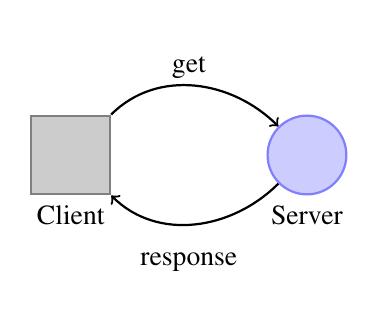
\begin{tikzpicture}
%        [server/.style={minimum size=10mm,circle,draw=blue!50,fill=blue!20,thick},
%        client/.style={minimum size=10mm,rectangle,draw=black!50,fill=black!20,thick}]
%        \node (S) at (9,4) [server, label=top:Server] {};
%        \node (C) at (6,4)[client, label=below:Client] {}
%        edge[<-, bend right=45] node[auto=right] {RESPONSE} (S)
%        edge[->, bend left=45] node[auto=right] {GET} (S) ;
%
        [server/.style={minimum size=10mm,circle,draw=blue!50,fill=blue!20,thick},
        client/.style={minimum size=10mm,rectangle,draw=black!50,fill=black!20,thick},
        arrow/.style={thick}]
        \node (server) at (9,4)[server, label=below:Server] {};
        \node (client) at (6,4)[client, label=below:Client] {};
%        \draw[red] (client) -> (server);
%        \draw[arrow] (server) edge[->,out=225,in=315] (client);
        \visible<2->{\path[arrow] (client) edge[->,out=45,in=135] (server);%
        \node (get) at (7.5,5.5)[label=below:get] {};}%
        \visible<3->{\path[arrow] (server) edge[->,out=225,in=315] (client);%
        \node (response) at (7.5,3)[label=below:response] {};}%
    \end{tikzpicture}\\%
\end{center}%
            \only<2-3>{\underline{get}: \texttt{\small{http://www.uniprot.org/uniprot/P12931} }}%
            \only<4>{\underline{get}: \texttt{\small{http://www.uniprot.org/uniprot/P12931\textbf{.txt}} }}%
            \only<3>{\\\underline{response}: \vspace{4mm}\textbf{HTML\\}%
            \optional{\includegraphics[height=.3\textheight]{images/uniprot_html.png}}%
%            \texttt{\small{%
%            <!DOCTYPE html>\\
%            <html xml:lang=``en'' xmlns=``http://www.w3.org/1999/xhtml''>\\
%            <head>\\
%            <title>UniProt</title>\\
%            <meta http-equiv=``X-UA-Compatible'' content=``IE=edge''>\\
%            <meta http-equiv=``Content-Type'' content=``text/html; charset=UTF-8''>\\
%            <link rel=``home'' href=``/''>\\
%            ... } 
            }%
            \only<4->{\\\underline{response:} \textbf{TEXT/TSV\\}%
            \vspace{4mm}\texttt{\footnotesize{%
            ID   SRC\_HUMAN               Reviewed;         536 AA.\\%
            AC   P12931; E1P5V4; Q76P87; Q86VB9; Q9H5A8;\\%
            DT   01-OCT-1989, integrated into UniProtKB/Swiss-Prot.\\%
            DT   23-JAN-2007, sequence version 3.\\%
            DT   03-SEP-2014, entry version 187.\\%
            DE   RecName: Full=Proto-oncogene tyrosine-protein kinase Src;\\%
            ... } }}%
\end{frame}


\section{REST}
\begin{frame}[t]\frametitle{\insertsection{}}
        \note{}
        \begin{block}{A RESTful application}
          is an application that exposes its state and functionality as a set of resources that the clients can manipulate and conforms to a certain set of principles:
          \begin{itemize}[<+->]
          \item All resources are uniquely addressable, usually through URIs; other addressing can also be used, though.
          \item All resources can be manipulated through a constrained set of well-known actions, usually CRUD (create, read, update,
            delete), represented most often through the HTTP's POST, GET, PUT and DELETE; it can be a different set or a subset
            though - for example, some implementations limit that set to read and modify only (GET and PUT) for example
          \item The data for all resources is transferred through any of a constrained number of well-known representations, usually HTML, XML or JSON;
          \item The communication between the client and the application is performed over a *stateless* protocol that allows for
            multiple layered intermediaries that can reroute and cache the requests and response packets transparently for the
            client and the application.
          \end{itemize}
        \end{block}
        \begin{center}
        \end{center}
\end{frame}

\section{REST Methods}
\begin{frame}[t]\frametitle{\insertsection{}}
\note{}
\begin{block}{}
\begin{description}{}
\item<+->[\alert<2>{Method}] defines what you want to do (\textbf{GET}=retrieve, \textbf{POST}=create/update, \textbf{DELETE}=remove).\\
    {\scriptsize We'll be using just GET requests which can be thought of as read-only access. POST/DELETE are used to modify data on a server.}
    %
    \item<+->[\alert<3>{URL}] defines a path to a resource
    %
    \item<+->[\alert<4>{Parameters}] additional arguments, filters etc. usually in the form $parameter=value$; the first parameter is separated from the url by '$?$' while subsequent ones use '$\&$'.
    \end{description}
    \end{block}
    \only<1->{%
      \begin{exampleblock}{Example: searching for the term 'EMBO':}
      \alert<1>{https}://\alert<2>{startpage.com/do/search}\alert<3>{?query=EMBO\&with\_language=lang\_de}
    \end{exampleblock}
    }
    \only<4->{\begin{alertblock}{Note:}
    For all these examples, any common browser can be used, however for proper 'programmatic' access
    tools such as 'curl' or 'wget' on the Linux/Mac commandline are much more efficient and can easily 
    be incorporated into little scripts...
    \end{alertblock}
    }
\end{frame}

\section{Benefits}
\begin{frame}[t]\frametitle{\insertsection{}}
\note{%
When in doubt whether a resource offers a REST interface search their help pages or google for "REST API", or "REST webservice"\\
Use a programmatic interface whenever possible. Write down the query you performed (best write it into a script file).
This way you'll have a protocol of what you've done and you can easily repeat these steps and thus update your results.
}
  \begin{description}[<+->]
   \item[Easy requests] The data can be requested with simple HTTP requests and returned in a variety of programatic and bioinformatical relevant formats such as JSON, XML, YAML and FASTA. 
   \item[Easy debugging] Debugging can be done in any browser. While some might not call this real programming, it surely is the first step towards programmatically querying resources.
   \item[Reproducable] You can write all your queries into a simple script and repeat the same query later. Even just saving the URL as a bookmark in your browser helps!
   \item[Powerful] Any data can be made available via a REST service.
   \item[Bandwidth] An API allows programmatic access to some information if one does not want to download the entire dataset.
   \item[Standards] By using existing protocols and best-methods (HTTP), all the existing knowledge can be reused (Caching, Redirecting, ...).
   \item[Widespread] More and more resource providers change from fat/heavy webservices to this lightweight system, for obvious reasons.
  \end{description}
  \vspace{-2mm}%
  \visible<8>{\begin{exampleblock}{Note:}
  Not meant to be a substitute for resources such as BioMART etc!
  \end{exampleblock}}
\end{frame}

\section{Example: Phospho.ELM}
\begin{frame}[t]\frametitle{\insertsection{}}
\note{You've already seen and used the Phospho.ELM database; queried it using the browser. Now we want to get results in a more structured way:}
\begin{center}
    \only<1|handout:0>{\optional{\includegraphics[height=.7\textheight]{images/Phospho_startpage_elm.png}}}%
    \only<2-|handout:1>{\optional{\includegraphics[height=.7\textheight]{images/Phospho_access_methods.png}}}\\%
\only<1>{http://phospho.elm.eu.org/index.html\\}%
\only<2>{http://phospho.elm.eu.org/byAccession/P55211.html\\}%
\only<3>{http://phospho.elm.eu.org/byAccession/P55211.{\color{red}csv}\\}%
\end{center}
\end{frame}

\begin{frame}[t,fragile]\frametitle{\insertsection{}}
    \note{~}
    \begin{center}
        \begin{alertblock}{Query}%
            http://phospho.elm.eu.org/\alert<2>{bySubstrate}/\alert<3>{cd66}.\alert<4>{html}%
            \visible<2->{\begin{itemize}
                \item<2-> \alert<2>{Query by Substrate name}
                \item<3-> \alert<3>{Substrate name}
                \item<4-> \alert<4>{Output as HTML}
            \end{itemize}}
        \end{alertblock}%
        Output:\\
        \only<1-|handout:1>{\optional{\includegraphics[height=.6\textheight]{images/phospho_output_substrate_html.png}}}%
    \end{center}
\end{frame}

\begin{frame}[t,fragile]\frametitle{\insertsection{}}
    \note{~}
    \begin{alertblock}{Query}%
        http://phospho.elm.eu.org/\alert<2>{byAccession}/\alert<3>{P12931}/\alert<4>{Pos12,17}.\alert<5>{csv}%
        \visible<2->{\begin{itemize}
            \item<2-> \alert<2>{query by Uniprot Accession}
            \item<3-> \alert<3>{Protein Sequence Accession/ID}
            \item<4-> \alert<4>{Position / multiple Positions}
            \item<5-> \alert<5>{Output as CSV (character separated values)}
        \end{itemize}}
    \end{alertblock}%
    Output:\\
    \hspace*{-1cm}
    \begin{semiverbatim}
    \scriptsize{
    \hspace*{-0.75cm}Acc.; Res.; Pos.; Context; Kinase; PMID; Source; ConScore; ELM; Domain; SMART; IUPRED; PDB; P3D-Acc;
    \hspace*{-0.75cm}\alert<3>{P12931}; S; \alert<4>{12}; SNKSKPKDASQRRRSLEPAE; none; 2136766; 1; 0.21; ; -; ; 0.9168; -; ;
    \hspace*{-0.75cm}\alert<3>{P12931}; S; \alert<4>{17}; PKDASQRRRSLEPAENVHGA; none; 18088087; 2; 0.24; MOD_PKA_1; -; ; 0.8828; -; ;
    \hspace*{-0.75cm}\alert<3>{P12931}; S; \alert<4>{17}; PKDASQRRRSLEPAENVHGA; none; 17192257; 2; 0.24; MOD_PKA_1; -; ; 0.8828; -; ;
    \hspace*{-0.75cm}\alert<3>{P12931}; S; \alert<4>{17}; PKDASQRRRSLEPAENVHGA; none; 17081983; 2; 0.24; MOD_PKA_1; -; ; 0.8828; -; ;
    \hspace*{-0.75cm}\alert<3>{P12931}; S; \alert<4>{17}; PKDASQRRRSLEPAENVHGA; PKA_group; 11804588; 1; 0.24; MOD_PKA_1; -; ; 0.8828; -; ;
    \hspace*{-0.75cm}...
    }
    \end{semiverbatim}%
\end{frame}

\section{Example: ELM}
\begin{frame}[t]\frametitle{\insertsection{}}
\note{}
\begin{center}
    \only<1|handout:1>{\optional{\includegraphics[width=\textwidth]{images/elm_instances1.png}}}\\
    \only<2|handout:0>{\optional{\includegraphics[width=\textwidth]{images/elm_instances2.png}}}\\
    \only<3|handout:0>{\optional{\includegraphics[width=\textwidth]{images/elm_downloads1.png}}}\\
    \only<4|handout:0>{\optional{\includegraphics[width=\textwidth]{images/elm_downloads2.png}}}\\
\end{center}
\end{frame}

\section{Example: STRING / STITCH}
\begin{frame}[t]\frametitle{\insertsection{}}
\note{}
\begin{center}
    \visible<1-|handout:1>{\hspace*{-0.55cm}\optional{\includegraphics[width=\textwidth]{images/string_api_format.png}}}\\
    \visible<2>{\hspace*{-0.55cm}\scriptsize{\verb |http://string-db.org/api/psi-mi-tab/interactions?identifier=YOL086C\&additional\_network\_nodes=2}}
\end{center}
\end{frame}

\section{Example: Uniprot}
\begin{frame}[t]\frametitle{\insertsection{}}
        \note{}
%        \only<1>{\begin{block}{Uniprot}
%        The Universal Protein Resource (UniProt) is a comprehensive resource for protein sequence and annotation data consisting of
%        the UniProt Knowledgebase (UniProtKB), the UniProt Reference Clusters (UniRef), and the UniProt Archive (UniParc) and more.
%        \end{block}}
        \begin{center}
            \only<1|handout:1>{\optional{\includegraphics[width=.99\textwidth]{images/Uniprot_Search_Abl.png}}}%
            \only<2|handout:0>{\optional{\includegraphics[width=.99\textwidth]{images/Uniprot_Download.png}}}%
%            \only<3|handout:0>{\vspace*{-0.45cm}\optional{\includegraphics[width=.99\textwidth]{images/Uniprot_Search_Advanced.png}}}%
        \end{center}
\end{frame}

\section{Questions?}
\begin{frame}<presentation:1|handout:0>[t]\frametitle{}
    \note{~}
    \begin{center}
      \vspace*{-0.5cm}\huge{Questions?}\\
        \optional{\includegraphics[height=.8\textheight]{images/question_kitten.jpg}}
    \end{center}
\end{frame}

\end{document}
